%%%%%%%%%%%%%%%%%%%%%%%%%%%%%%%%%%%%%%%%%
% Beamer Presentation
% LaTeX Template
% Version 1.0 (10/11/12)
%
% This template has been downloaded from:
% http://www.LaTeXTemplates.com
%
% License:
% CC BY-NC-SA 3.0 (http://creativecommons.org/licenses/by-nc-sa/3.0/)
%
%%%%%%%%%%%%%%%%%%%%%%%%%%%%%%%%%%%%%%%%%

%----------------------------------------------------------------------------------------
%	PACKAGES AND THEMES
%----------------------------------------------------------------------------------------

\documentclass{beamer}

\mode<presentation> {

% The Beamer class comes with a number of default slide themes
% which change the colors and layouts of slides. Below this is a list
% of all the themes, uncomment each in turn to see what they look like.

%\usetheme{default}
%\usetheme{AnnArbor}
%\usetheme{Antibes}
%\usetheme{Bergen}
%\usetheme{Berkeley}
%\usetheme{Berlin}
%\usetheme{Boadilla}
%\usetheme{CambridgeUS}
%\usetheme{Copenhagen}
%\usetheme{Darmstadt}
%\usetheme{Dresden}
%\usetheme{Frankfurt}
%\usetheme{Goettingen}
%\usetheme{Hannover}
%\usetheme{Ilmenau}
%\usetheme{JuanLesPins}
%\usetheme{Luebeck}
\usetheme{Madrid}
%\usetheme{Malmoe}
%\usetheme{Marburg}
%\usetheme{Montpellier}
%\usetheme{PaloAlto}
%\usetheme{Pittsburgh}
%\usetheme{Rochester}
%\usetheme{Singapore}
%\usetheme{Szeged}
%\usetheme{Warsaw}

% As well as themes, the Beamer class has a number of color themes
% for any slide theme. Uncomment each of these in turn to see how it
% changes the colors of your current slide theme.

%\usecolortheme{albatross}
%\usecolortheme{beaver}
%\usecolortheme{beetle}
%\usecolortheme{crane}
%\usecolortheme{dolphin}
%\usecolortheme{dove}
%\usecolortheme{fly}
%\usecolortheme{lily}
%\usecolortheme{orchid}
%\usecolortheme{rose}
%\usecolortheme{seagull}
%\usecolortheme{seahorse}
%\usecolortheme{whale}
%\usecolortheme{wolverine}

%\setbeamertemplate{footline} % To remove the footer line in all slides uncomment this line
%\setbeamertemplate{footline}[page number] % To replace the footer line in all slides with a simple slide count uncomment this line

\setbeamertemplate{navigation symbols}{} % To remove the navigation symbols from the bottom of all slides uncomment this line
}

\usepackage{hyperref}
\usepackage{graphicx} % Allows including images
\usepackage{booktabs} % Allows the use of \toprule, \midrule and \bottomrule in tables
\newcommand{\shellcmd}[1]{'\texttt{\footnotesize #1}'}
\newcommand{\shellcmdtiny}[1]{'\texttt{\scriptsize #1}'}
%----------------------------------------------------------------------------------------
%	TITLE PAGE
%----------------------------------------------------------------------------------------

\title[Git]{A short intro to Git} % The short title appears at the bottom of every slide, the full title is only on the title page

\author{Thomas Moreau} % Your name
\institute[CMLA] % Your institution as it will appear on the bottom of every slide, may be shorthand to save space
{
Centre de mathématiques et de leur applications \\ % Your institution for the title page
ENS Cachan\\
\medskip
\textit{thomas.moreau@cmla.ens-cachan.fr} % Your email address
}
\date{\today} % Date, can be changed to a custom date

\begin{document}

\begin{frame}
\titlepage % Print the title page as the first slide
\end{frame}

%----------------------------------------------------------------------------------------
%	PRESENTATION SLIDES
%----------------------------------------------------------------------------------------


\begin{frame}
\frametitle{Versioning}
\begin{itemize}
\item Open source project
\item Keep track of code changes
\item Good to collaborate with code
\end{itemize}
\begin{figure}[htp]
\centering
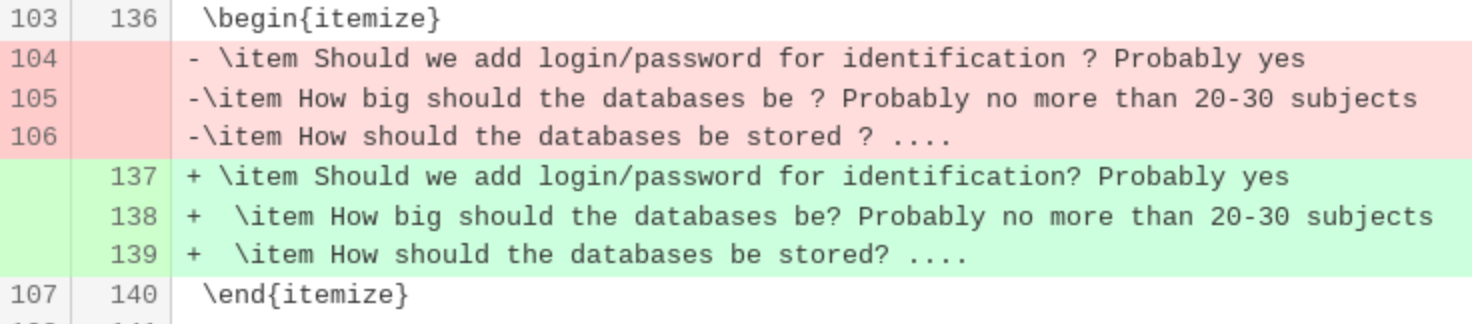
\includegraphics[width=\textwidth]{diff.png}
\label{}
\end{figure}

\centering
Really good at comparing lines!

\end{frame}


\begin{frame}
	\frametitle{Vocabulary}
	\begin{itemize}
    	\item Repository: The whole collaborative project
    	\item Local: The local version of the code
    	\item Remote: Server side tracker
    	\item Commit: Chunk of code
    	\item Branch: Succession of commit
    	\item Origin: Default remote tracker
    	\item Master: Default branch
    	\item HEAD:   Current version of the code
    \end{itemize}
\end{frame}

\begin{frame}
    \frametitle{Commit}
    Useful for packaging changes:
    \begin{itemize}
	    \item \shellcmd{git add FILES}: add FILES to the next commit
	    \item \shellcmd{git commit [-m msg]}: create a commit - add a meaningful message
    \end{itemize}
    \begin{figure}[htp]
    \centering
    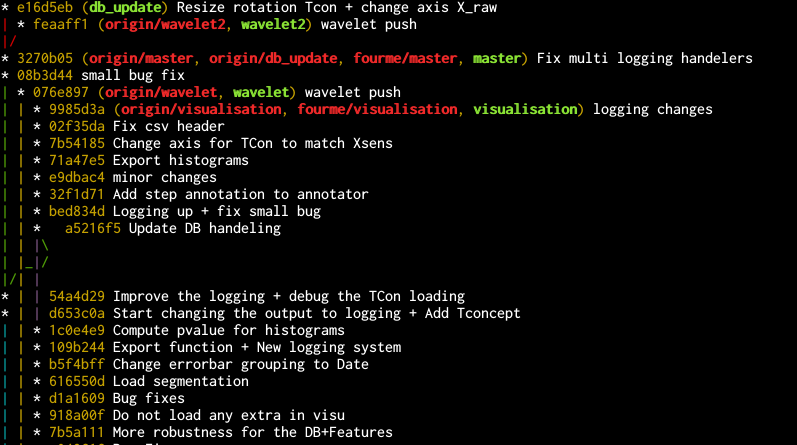
\includegraphics[width=\textwidth]{commit}
    \end{figure}
\end{frame}

\begin{frame}
	\frametitle{Status}
	Information about the state of the repository
    \begin{figure}[htp]
        \centering
        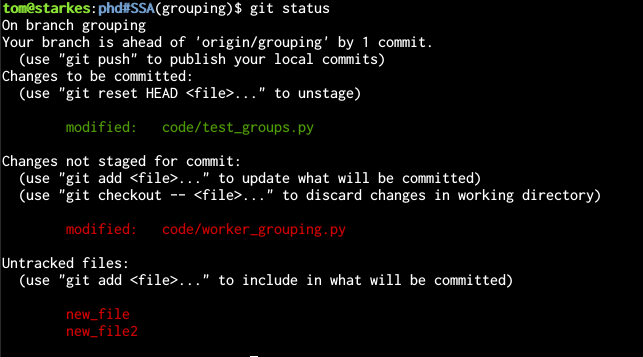
\includegraphics[width=\textwidth]{status}
    \end{figure}
\end{frame}

\begin{frame}
	\frametitle{Interacting with other}
	\begin{tabular}{l c l}
	    \shellcmd{git push} &$\rightarrow$ &Upload changes to remote repo\\
        \shellcmd{git pull} &$\rightarrow$ &Get changes from remote repo\\
	\end{tabular}
	\\\vspace{.8cm}
	Automatic merging of the files that have been modified on both sides:\\
	\begin{itemize}
	\item fetch changes
	\item Put the 2 codes together either by merging or rebasing
	\item 
\end{itemize}
	Another possibility \shellcmd{git fetch; git rebase origin/BRANCH}
	
\end{frame}

\begin{frame}
	\frametitle{Introduction to branching}
    \href{http://k.swd.cc/learnGitBranching-ja/?NODEMO}{Demo}\\\vspace{1cm}
    
    Good practice:
	\begin{itemize}
	    \item Before working, pull changes
	    \item Use \shellcmd{git pull --rebase} to avoid unecessary commits\\
        \footnotesize{can be automatized with \shellcmdtiny{git config branch.autosetuprebase always}}
        \item \normalsize Better to have a branch per feature
    \end{itemize}
\end{frame}


\begin{frame}
	\frametitle{Conflict}
	
	Automatic merging can fail.\\
	
	Merge but put 
	\begin{figure}[htp]
\centering
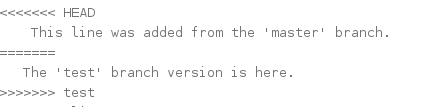
\includegraphics[scale=0.5]{conflict}
\end{figure}
	Manual resolution is needed and important to do first
\end{frame}


\begin{frame}
	\frametitle{Conclusion}
	Git
	\begin{itemize}
	\item status: know what is going on
	\item add/commit: create a chunk of code
	\item push: Send new commits to remote
	\item pull: Get the changes
	\item stash: put your changes on hold\\stash pop to get it back
\end{itemize}
\end{frame}

%------------------------------------------------

\begin{frame}
\Huge{\centerline{Questions?}}
\end{frame}

%----------------------------------------------------------------------------------------

\end{document} 